\chapter{Test}

%
%
%
\section{Jest}

Ogni microservizio definisce degli \emph{Unit Testing} mediante \emph{Jest} in modo da verificare la correttezza delle richieste e delle relative risposte, dei singoli microservizi.

In questo modo, siamo stati in grado di concentrarci sui seguenti aspetti durante i test:

\begin{itemize}
    \item Verifica della correttezza delle richieste fornite.

    \item Verifica della correttezza delle risposte fornite da diverse richieste.

    \item Test di integrazione per garantire che i vari endpoint si comportino correttamente, potendo verificare i side effect di una richiesta, eseguendo richieste successive.
\end{itemize}

Questo approccio ci ha permesso di sviluppare test solidi e garantire che i microservizi rispettassero gli standard richiesti.

%
%
%
\section{Microservizi}

Tutti i microservizi posseggono una suite di test.
%
Di seguito un esempio con il core del testing del servizio degli utenti:

\begin{lstlisting}[style=typescript, caption={microservice Test}, label=lst:login:route:test]
const userMicroservice: Microservice = new Microservice(UserServiceConfiguration)
let request: supertest.SuperTest<supertest.Test>

beforeAll(async () => {
  await userMicroservice.start()
  request = supertest(userMicroservice.getServer())
})

afterAll(async () => {
  await userMicroservice.stop()
})

afterEach(async () => {
  await userMicroservice.clearDatabase()
})

describe('Register', () => {
  it('A user must provide username, password and email', async () => {
    let response = await request
      .post('/auth/register')
      .send({ username: 'test', password: 'test' })
    expect(response.status).toBe(400)
    // other test stuff
    response = await request
      .post('/auth/register')
      .send({ username: 'test', password: 'test', email: 'test' })
    expect(response.status).toBe(200)
  })
    // other test stuff
})

describe('Login', () => {
    it('A user should provide username and password to login', async () => {
        let response = await register('test', 'test', 'test')
        response = await request.post('/auth/login').send({ username: 'test' })
        expect(response.status).toBe(400)
        response = await request.post('/auth/login').send({ password: 'test' })
        expect(response.status).toBe(400)
        response = await request
          .post('/auth/login')
          .send({ username: 'test', password: 'test' })
        expect(response.status).toBe(200)
    })
    // other test stuff
})

describe('Logout', () => {
  it('A user should be able to logout', async () => {
    let response = await createUserAndLogin('test', 'test', 'test')
    const cookie = response.header['set-cookie']
    response = await request.post('/auth/logout').set('Cookie', cookie)
    expect(response.status).toBe(200)
  })
    // other test stuff
})

describe('Refresh token', () => {
  it('A user should be able to refresh token', async () => {
    let response = await createUserAndLogin('test', 'test', 'test')
    const cookie = response.header['set-cookie']
    response = await request.post('/auth/refresh-token').set('Cookie', cookie)
    expect(response.status).toBe(200)
    expect(response.header['set-cookie']).toHaveLength(1)
  })
    // other test stuff
})

\end{lstlisting}

%
%
%
\section{Utenti}

Il sito è stato messo a disposizione di diversi gruppi di utenti per valutarne l'utilizzo e raccogliere feedback.
%
Questa fase di test è stata cruciale per valutare la facilità d'uso e comprendere come migliorare l'esperienza complessiva degli utenti.
%
Dopo l'utilizzo, è stato chiesto loro di compilare un Google Form, consentendo di raccogliere opinioni e osservazioni dirette.

Attraverso questo processo, siamo stati in grado di individuare aree che richiedono miglioramenti e identificare possibili bug che non erano emersi durante lo sviluppo iniziale.
%
I feedback degli utenti hanno fornito preziose informazioni su aspetti che possono essere ottimizzati per garantire un'esperienza più fluida e soddisfacente.

\begin{figure}[htbp]
    \centering
    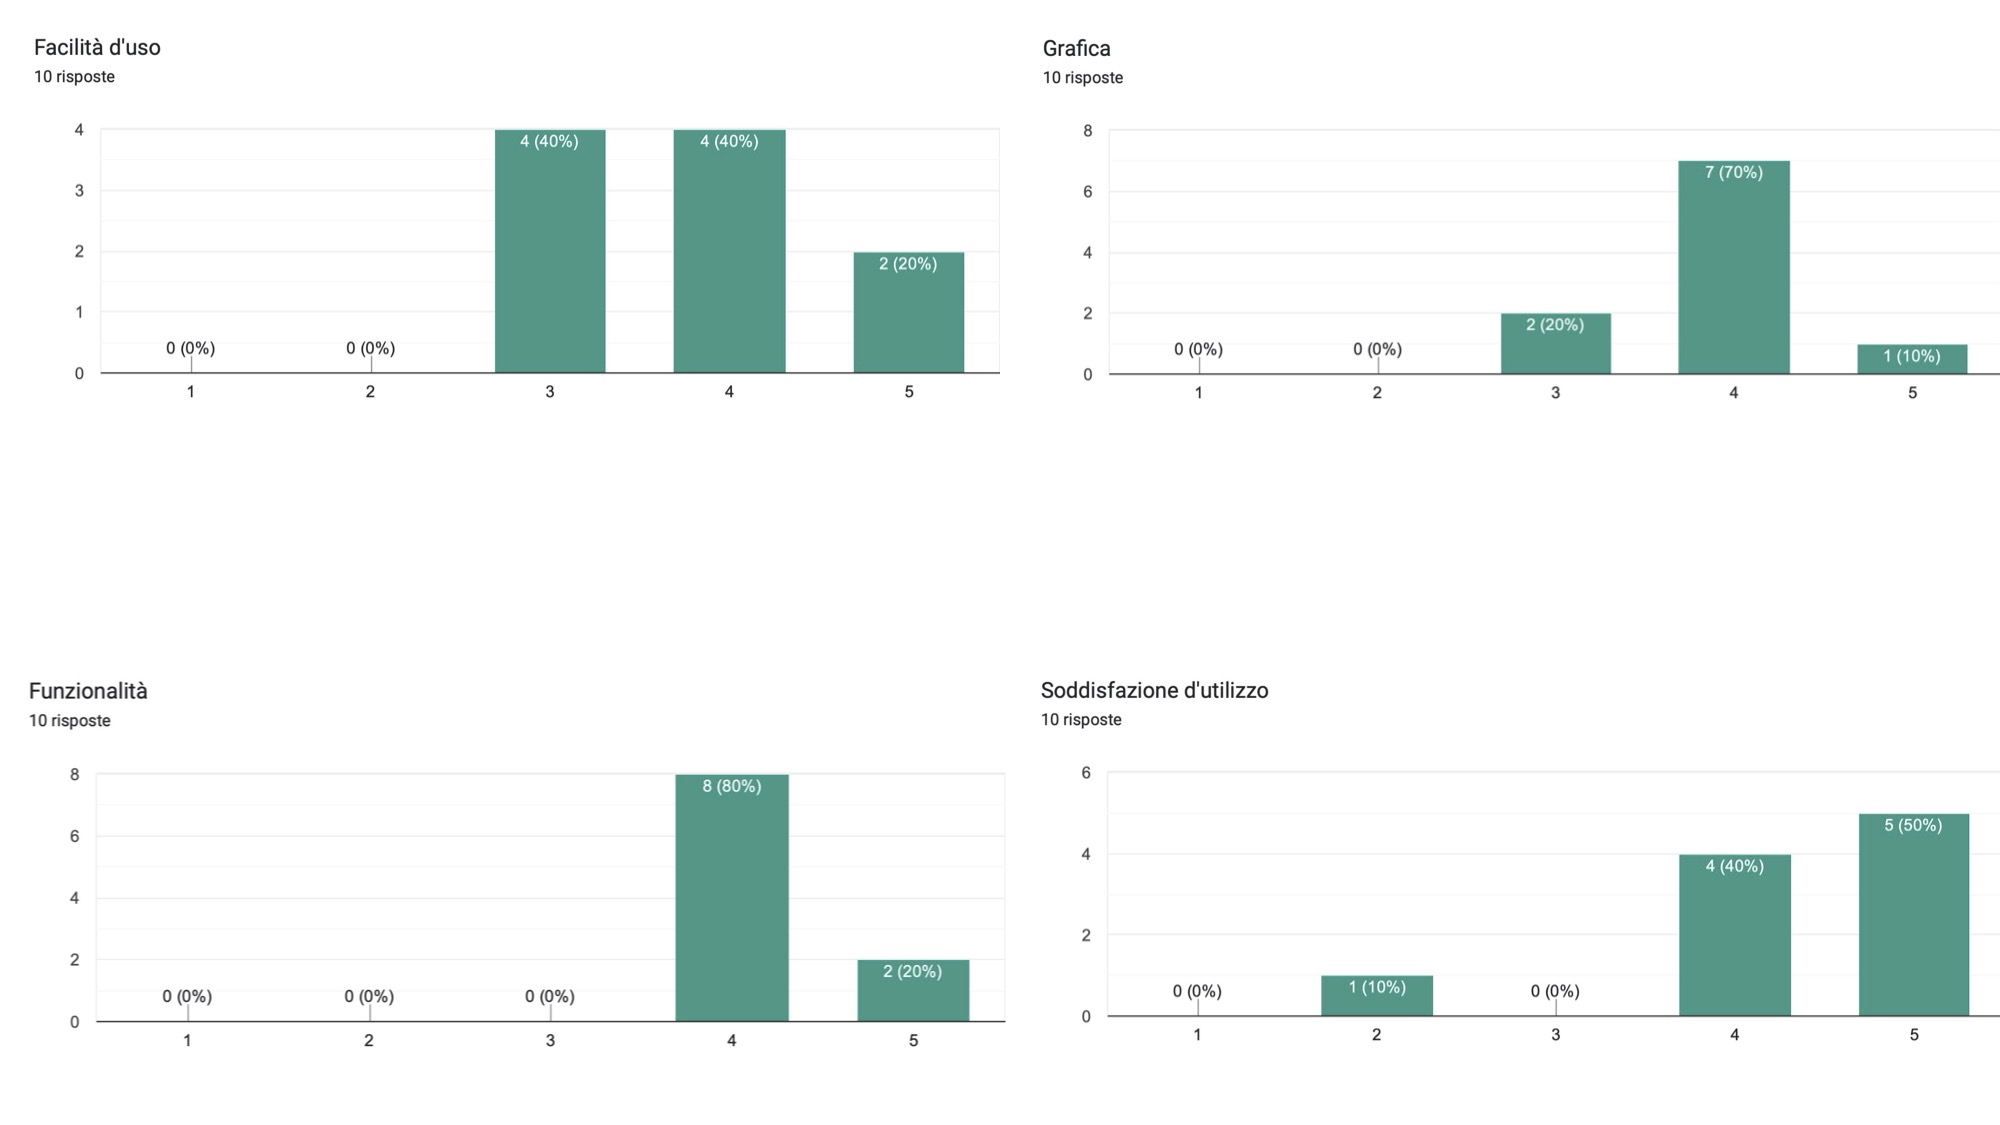
\includegraphics[width=\textwidth]{img/GraficiUtenti.jpg}
    \caption{Grafici del questionario rivolto agli utenti}
    \label{fig:grafico_user_expirience}
\end{figure}

\textbf{Grafica:}
    Abbiamo ricevuto una valutazione media di 3,8 su 5 per l'aspetto visivo del nostro prodotto. Le valutazioni variano da 3 a 5. La maggior parte degli utenti sembra apprezzare l'aspetto visuale, sebbene alcuni suggeriscano possibili miglioramenti.

\textbf{Facilità d'uso:}
    L'usabilità ha ottenuto una valutazione media di 3,5 su 5, con valutazioni comprese tra 3 e 5. Alcuni utenti potrebbero aver riscontrato difficoltà nell'utilizzo del sistema, indicando la necessità di miglioramenti per rendere il sistema più accessibile.
    
\textbf{Funzionalità:}
    Abbiamo ottenuto una valutazione media di 4,1 su 5 per le funzionalità offerte. La maggior parte degli utenti sembra apprezzare le funzionalità del nostro sistema, anche se ci sono alcune valutazioni più basse che indicano un gruppo di utenti che sente la necessità di un' esperienza più ampia.
    
\textbf{Soddisfazione d'utilizzo:}
    La soddisfazione media è di 4,3 su 5. La maggior parte degli utenti sembra essere soddisfatta dell'esperienza complessiva, tuttavia vi sono alcune valutazioni più basse che potrebbero indicare potenziali aree di miglioramento.

In generale, i punteggi più elevati sono stati attribuiti alla `Soddisfazione d'utilizzo' e alle `Funzionalità', mentre la `Grafica' e la `Facilità d'uso' presentano valutazioni più variabili.
%
Questi risultati ci offrono un'idea del livello di apprezzamento per il nostro prodotto e allo stesso tempo ci indicano dove concentrare gli sforzi per migliorare, specialmente riguardo all'usabilità e all'aspetto visivo, al fine di offrire un'esperienza più coerente e soddisfacente per tutti gli utenti.

%
%
%
\section{Accessibilità}

Per testare i requisiti di accessibilità abbiamo utilizzato lo strumento integrato in Safari, il quale analizzando l'applicazione ci ha fornito il seguente feedback:

\begin{figure}[H]
    \centering
    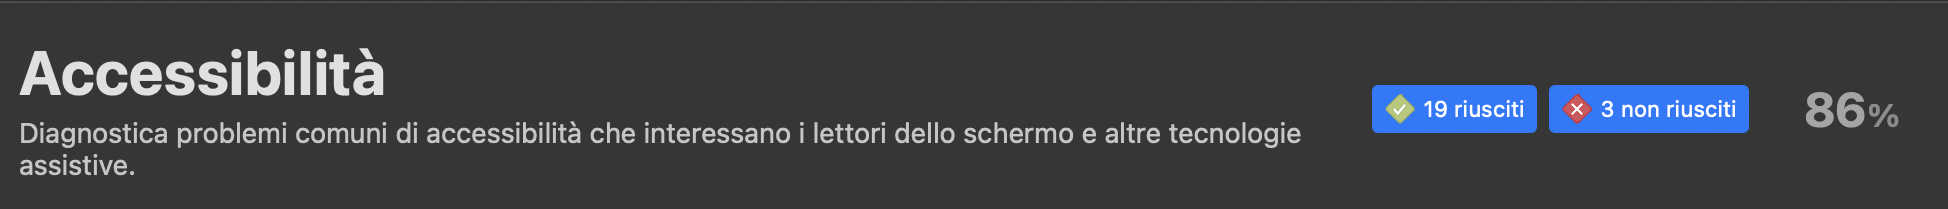
\includegraphics[width=1\textwidth]{img/accessibility.png}
    \caption{Test d'accessibilità di Safari}
    \label{fig:mockup-accessibility}
\end{figure}

Come possiamo notare non tutti i test hanno riscontrato un feedback positivo, tuttavia, alcuni di questi dipendono da Quasar, ovvero il framework utilizzato per lo sviluppo dei componenti, in relazione a ciò abbiamo dovuto trovare dei compromessi.
%
L'impiego di layout innestati ha generato dei conflitti che si sono rivelati piuttosto complessi da risolvere.
%
La combinazione di questi layout ha causato problemi che, purtroppo, non sono stati facilmente gestibili a causa delle restrizioni intrinseche del framework.
%
Abbiamo cercato soluzioni alternative, ma gli ostacoli persistenti hanno richiesto più tempo del previsto per essere affrontati in modo efficace.
